\subsection{csim-ref 命令行参数}
我们先要知道csim-ref的部分命令,以便于后续进行实验
\begin{itemize}
    \item -h:可选的帮助标志,用于打印使用情况信息
    \item -v:显示跟踪信息的可选详细标志
    \item -s <s>:设置的索引位数(S = 2s是设置的数量)
    \item -E <E>:关联性(每组行数)
    \item -b <b>:块位数(B = 2b是块大小)
    \item -t <tracefile>:要重播的valgrind跟踪的名称
    \item Usage: ./csim-ref [-hv] -s <s> -E <E> -b <b> -t <tracefile>
\end{itemize}

\subsection{模拟缓存行}
首先,我们先了解cache的结构:
\begin{itemize}
    \item cache一般分为S组,每组有E块
    \item 每块结构为一个有效位v,一个标志位tag,一个数据块data
    \item cache地址分为三部分:标志位tag,组索引s,块偏移b
\end{itemize}

根据缓存行相关的知识,我们定义了一个结构体,用于模拟缓存行的结构。

\begin{lstlisting}[language = C , title = { Struct Definition } ]
    typedef struct {
        int valid; // 有效位
        ulong tag; // 标志位
        clock_t time; // 时间
    } CacheLine;
\end{lstlisting}

通过二维数组的模拟,我们可以模拟cache的行为。

根据官方文档中的介绍,可以用 getopt() 函数来解析参数。

\begin{lstlisting}[language = C , title = { Getopt Function } ]
    int main(int argc, char** argv){
        int opt,x,y;
        /* looping over arguments */
        while((opt = getopt(argc, argv, “x:y:")) != -1){ // getopt() 函数解析参数
        /* determine which argument it’s processing */ // 确定正在处理的参数
        switch(opt) { // 判断参数
            case 'x':
                x = atoi(optarg); // 将参数转换为整数
                break;
            case ‘y':
                y = atoi(optarg); 
                break;
            default:
                printf(“wrong argument\n"); // 参数错误
                break;
            }
        }
    }
\end{lstlisting}

\subsection{代码实现}
首先要分配内存,然后初始化cache行,最后模拟cache的行为。

\subsubsection{分配内存}

\begin{lstlisting}[language = C , title = { Allocate Memory} ]
// 为缓存动态分配内存
CacheHead CacheInit(int S, int E) { 
	CacheHead cache; // 定义缓存
	cache = calloc(1 << S, sizeof(CacheSet)); // 分配内存

	if (cache == NULL) {
		printf("Fail to allocate memory for cache.\n"); // 分配内存失败
		exit(EXIT_FAILURE);
	}

	int i = 0; // 初始化
	for (i = 0; i < 1 << S; i++) { 
		if ((cache[i] = calloc(E, sizeof(CacheLine))) == NULL) {  // 分配内存
			printf("Fail to allocate memory for cache.\n"); 
			exit(EXIT_FAILURE); // 分配内存失败
		}
	}

	for (i = 0; i < 1 << S; i++) {
		int j;
		for (j = 0; j < E; j++) { 
			cache[i][j].valid = 0; // 有效位
		}
	}
	return cache;
}
\end{lstlisting}

\subsubsection{判断缓存状态}
\begin{lstlisting}[language = C , title = { Judge The Situation Of Cache} ]
// 判断缓存状态,是否有效,标记匹配
int CacheJudge(CacheHead cache, ulong index, ulong tag) {
	int i;
	int fullFlag = 1; // 标记是否满
	int matchFlag = 0;
	for (i = 0; i < globalOptions.associativity; i++) { 
		if (cache[index][i].valid == 0) { // 有效位为0
			fullFlag = 0;
		}
		if (cache[index][i].tag == tag && cache[index][i].valid == 1) { // 有效位为1
			matchFlag = 1;
		}
	}
	if (matchFlag == 1) // 匹配
		return CACHED; 
	if (fullFlag == 1)
		return NEED_EVICT; // 需要驱逐
	else
		return NO_MATCH; // 不匹配
}
\end{lstlisting}

\subsubsection{执行 eviction 操作}
\begin{lstlisting}[language = C , title = {Eviction} ]
// 判断缓存状态,是否有效,标记匹配
void CacheEvict(CacheHead cache, ulong index, ulong tag) { // 驱逐
	int firstLine = 0, i = 0;
	clock_t firstCachedTime = cache[index][i].time; // 时间
	for (i = 0; i < globalOptions.associativity; i++) { // 遍历
		if (cache[index][i].time < firstCachedTime) { // 时间比较
			firstCachedTime = cache[index][i].time; // 更新时间
			firstLine = i;
		}
	}
	CacheLine *target = cache[index] + firstLine; // 目标
	target->tag = 0; // 标志位
	target->time = 0; // 时间
	target->valid = 0; // 有效位
}
\end{lstlisting}

\subsubsection{执行读取操作}
\begin{lstlisting}[language = C , title = {Cache Touch} ]
// 执行读取的操作
void CacheTouch(CacheHead cache, ulong index, ulong tag) {
	int touchLine = 0; // 读取
	while (cache[index][touchLine].tag != tag) { // 标志位不匹配
		touchLine++; // 读取下一行
	}
	cache[index][touchLine].time = clock(); // 更新时间
}
\end{lstlisting}

\subsubsection{执行写入缓存操作}
\begin{lstlisting}[language = C , title = {Cache Insert} ]
// 写入缓存
void CacheInsert(CacheHead cache, ulong index, ulong tag) {
	int freeLine = 0, i;
	for (i = 0; i < globalOptions.associativity; i++) {
		if (cache[index][i].valid == 0) // 有效位为0
			break; // 跳出循环
		freeLine++; // 空行
	}
	CacheLine *target = cache[index] + freeLine; // 目标
	target->tag = tag;  // 标志位
	target->valid = 1;	// 有效位为1
	target->time = clock(); // 更新时间
}
\end{lstlisting}

\subsubsection{计数器}
\begin{lstlisting}[language = C , title = {Counter} ]
// 计数器,增加 hit, miss 和 eviction 的数量
void Adder(int type, int num) {
	int v = globalOptions.verboseFlag; // 详细标志
	switch (type) {
	case ADD_EVICT:
		totalEvictCount += num; // 驱逐
		if (v && num != 0) // 详细标志
			printf("eviction ");
		break;
	case ADD_HIT:
		totalHitCount += num; // 命中
		if (v && num != 0) // 详细标志
			printf("hit ");
		break;
	case ADD_MISS:
		totalMissCount += num; // 未命中
		if (v && num != 0) // 详细标志
			printf("miss ");
	}
}
\end{lstlisting}

\subsubsection{打印内存数据}
\begin{lstlisting}[language = C , title = {Print Byte} ]
// 逐字节以 16 进制打印内存数据
void printByte(bytept h, int len) {
	int i;
	for (i = 0; i < len; i++)
		printf("%.2x ", h[i]); // 逐字节打印
	printf("\n");
}
\end{lstlisting}

\subsubsection{主要执行函数}
\begin{lstlisting}[language = C , title = {Execute Function} ]
void Execute(CacheHead cache, char type, ulong address, int len) {
    ulong index = (address << globalOptions.tagBits) >> (MACHINE_BITS - globalOptions.setIndexBits); // 索引
    ulong tag = address >> (globalOptions.blockBits + globalOptions.setIndexBits); // 标志
    int status = CacheJudge(cache, index, tag); // 判断
    if (globalOptions.verboseFlag == 1) {
        if(globalOptions.superVerboseFlag == 1){
            printf("\n[address:] ");
            printByte((bytept)&address, sizeof(long)); // 打印内存数据
            printf("[index:] ");
            printByte((bytept)&index, sizeof(long));
            printf("[tag:] ");
            printByte((bytept)&tag, sizeof(long));
            printf("(Decimal)[index: %ld, tag: %ld]\n------------------------------------------- ", index, tag);
        } 
        else{
            printf("(Decimal)[index: %ld, tag: %ld] ------ ", index, tag);
        }
    }
    switch (status) { // 判断状态
    case CACHED:
        CacheTouch(cache, index, tag); // 读取
        if (type == 'M') {
            Adder(ADD_HIT, 1); // 命中
            Adder(ADD_HIT, 1);
        } else {
            Adder(ADD_HIT, 1);
        }
        break;
    case NO_MATCH:
        CacheInsert(cache, index, tag); // 写入
        if (type == 'M') {
            Adder(ADD_MISS, 1);
            Adder(ADD_HIT, 1);
        } else {
            Adder(ADD_MISS, 1);
        }
        break;
    case NEED_EVICT:
        CacheEvict(cache, index, tag); // 驱逐
        CacheInsert(cache, index, tag); // 写入
        if (type == 'M') {
            Adder(ADD_MISS, 1);
            Adder(ADD_EVICT, 1);
            Adder(ADD_HIT, 1);

        } else {
            Adder(ADD_MISS, 1);
            Adder(ADD_EVICT, 1);
        }
        break;
    default:
        printf("Unknown error.\n");
        exit(EXIT_FAILURE);
    }
    if (globalOptions.verboseFlag == 1) {
        printf("\n");
    }
}

\end{lstlisting}

\subsubsection{驱动函数}
\begin{lstlisting}[language = C , title = {Main} ]
// 读取参数,打开文件
int main(int argc, char *args[]) {
	char ch;
	while ((ch = getopt(argc, args, optString)) != -1) {
		switch (ch) {
		case 's':
			if (atoi(optarg) < 0) {
				printf("Unvalid input for <s>. Try Again.\n"); // 无效输入
				exit(EXIT_FAILURE); // 退出
			}
			globalOptions.setIndexBits = atoi(optarg); // 索引位数
			break;
		case 'E':
			if (atoi(optarg) < 0) {
				printf("Unvalid input for <E>. Try Again.\n"); // 无效输入
				exit(EXIT_FAILURE); // 退出
			}
			globalOptions.associativity = atoi(optarg); // 关联性
			break;
		case 'b':
			if (atoi(optarg) < 0) {
				printf("Unvalid input for <b>. Try Again.\n"); // 无效输入
				exit(EXIT_FAILURE); // 退出
			}
			globalOptions.blockBits = atoi(optarg); // 块位数
			break;
		case 't':
			globalOptions.traceDir = optarg; // 跟踪文件
			break; 
		case 'v':
			globalOptions.verboseFlag = 1; // 详细标志
			break;
		case 'h':
			usage();
			exit(EXIT_FAILURE); // 退出
		case 'V':
			globalOptions.verboseFlag = 1; // 详细标志
			globalOptions.superVerboseFlag = 1; // 详细标志
			break;
		default:
			usage(); // 使用
			exit(EXIT_FAILURE); // 退出
			break;
		}
	}
	globalOptions.tagBits = MACHINE_BITS - globalOptions.blockBits - globalOptions.setIndexBits; // 标志位

	FILE *traceFile = fopen(globalOptions.traceDir, "r"); // 打开文件
	if (traceFile == NULL) {
		printf("Fail to open file: %s\n", globalOptions.traceDir); // 打开文件失败
		exit(EXIT_FAILURE);
	}
	CacheHead cache = CacheInit(globalOptions.setIndexBits, globalOptions.associativity); // 初始化
	char traceLine[32];
	while (fgets(traceLine, 32, traceFile) != NULL) { // 读取文件
		char mode; // 模式
		ulong address; // 地址
		int len; // 长度
		sscanf(traceLine, " %c %lx,%d", &mode, &address, &len); // 读取
		if (mode == 'I')
			continue;
		if (globalOptions.verboseFlag == 1) {
			printf("%c %lx,%d ", mode, address, len); // 打印
		}
		Execute(cache, mode, address, len); // 执行
	}
	printSummary(totalHitCount, totalMissCount, totalEvictCount); // 打印结果
	free(cache);
	return 0;
}
\end{lstlisting}

\subsubsection{基本参数}
\begin{lstlisting}[language = C , title = {Parameter Definition} ]
#define MACHINE_BITS 64 // 机器位数
#define NEED_EVICT -1 // 需要驱逐
#define NO_MATCH -2 // 不匹配
#define CACHED 1 // 命中
#define ADD_HIT 1 // 增加命中
#define ADD_MISS 2 // 增加未命中
#define ADD_EVICT 3 // 增加驱逐

int totalMissCount = 0; // 未命中
int totalHitCount = 0; // 命中
int totalEvictCount = 0; // 驱逐

typedef unsigned long ulong; // 无符号长整型
typedef unsigned char *bytept; // 无符号字符型指针
const char *optString = "s:E:b:t:hVv"; 

struct globalOptions {
	int setIndexBits; // 索引位数
	int associativity; // 关联性
	int blockBits; // 块位数
	int verboseFlag; // 详细标志
	int tagBits; // 标志位
	int superVerboseFlag; // 详细标志
	char *traceDir; // 跟踪文件
} globalOptions;

struct result {
	int hit; // 命中
	int miss; // 未命中
	int evict; // 驱逐
};

typedef struct {
	int valid;
	ulong tag;
	clock_t time;
} CacheLine;

typedef CacheLine *CacheSet; // 缓存行
typedef CacheSet *CacheHead; // 缓存头
\end{lstlisting}

\subsection{实验结果}
我们使用 $ csim-ref $ 来测试我们的代码:
将在Windows下编译好的文件放入Linux系统中,然后使用make clean 和 make来编译,最后
使用 $./test-csim$ 运行测试,结果如下:

\begin{figure} [H]
    \centering
    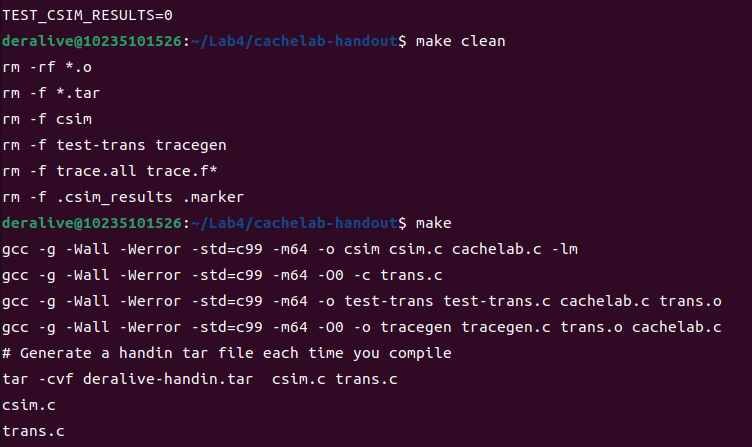
\includegraphics[width=0.4\textwidth]{Make.png}
    \caption{Makefile 编译成功}
\end{figure}

\begin{figure} [H]
    \centering
    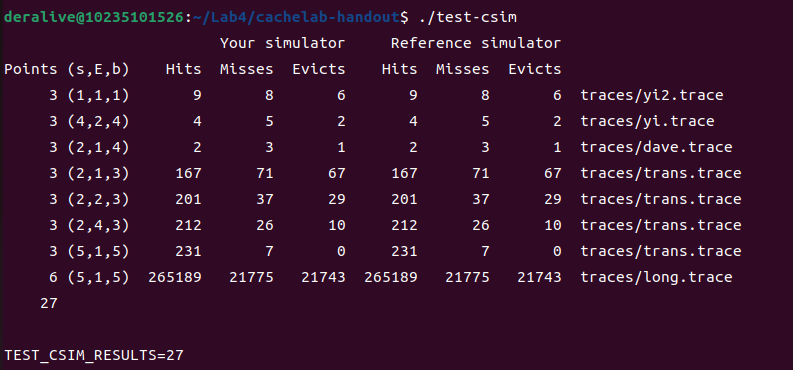
\includegraphics[width=0.5\textwidth]{csim.png}
    \caption{跑分结果}
\end{figure}